% !TEX root = ../../main.tex


\begin{figure}[tb]
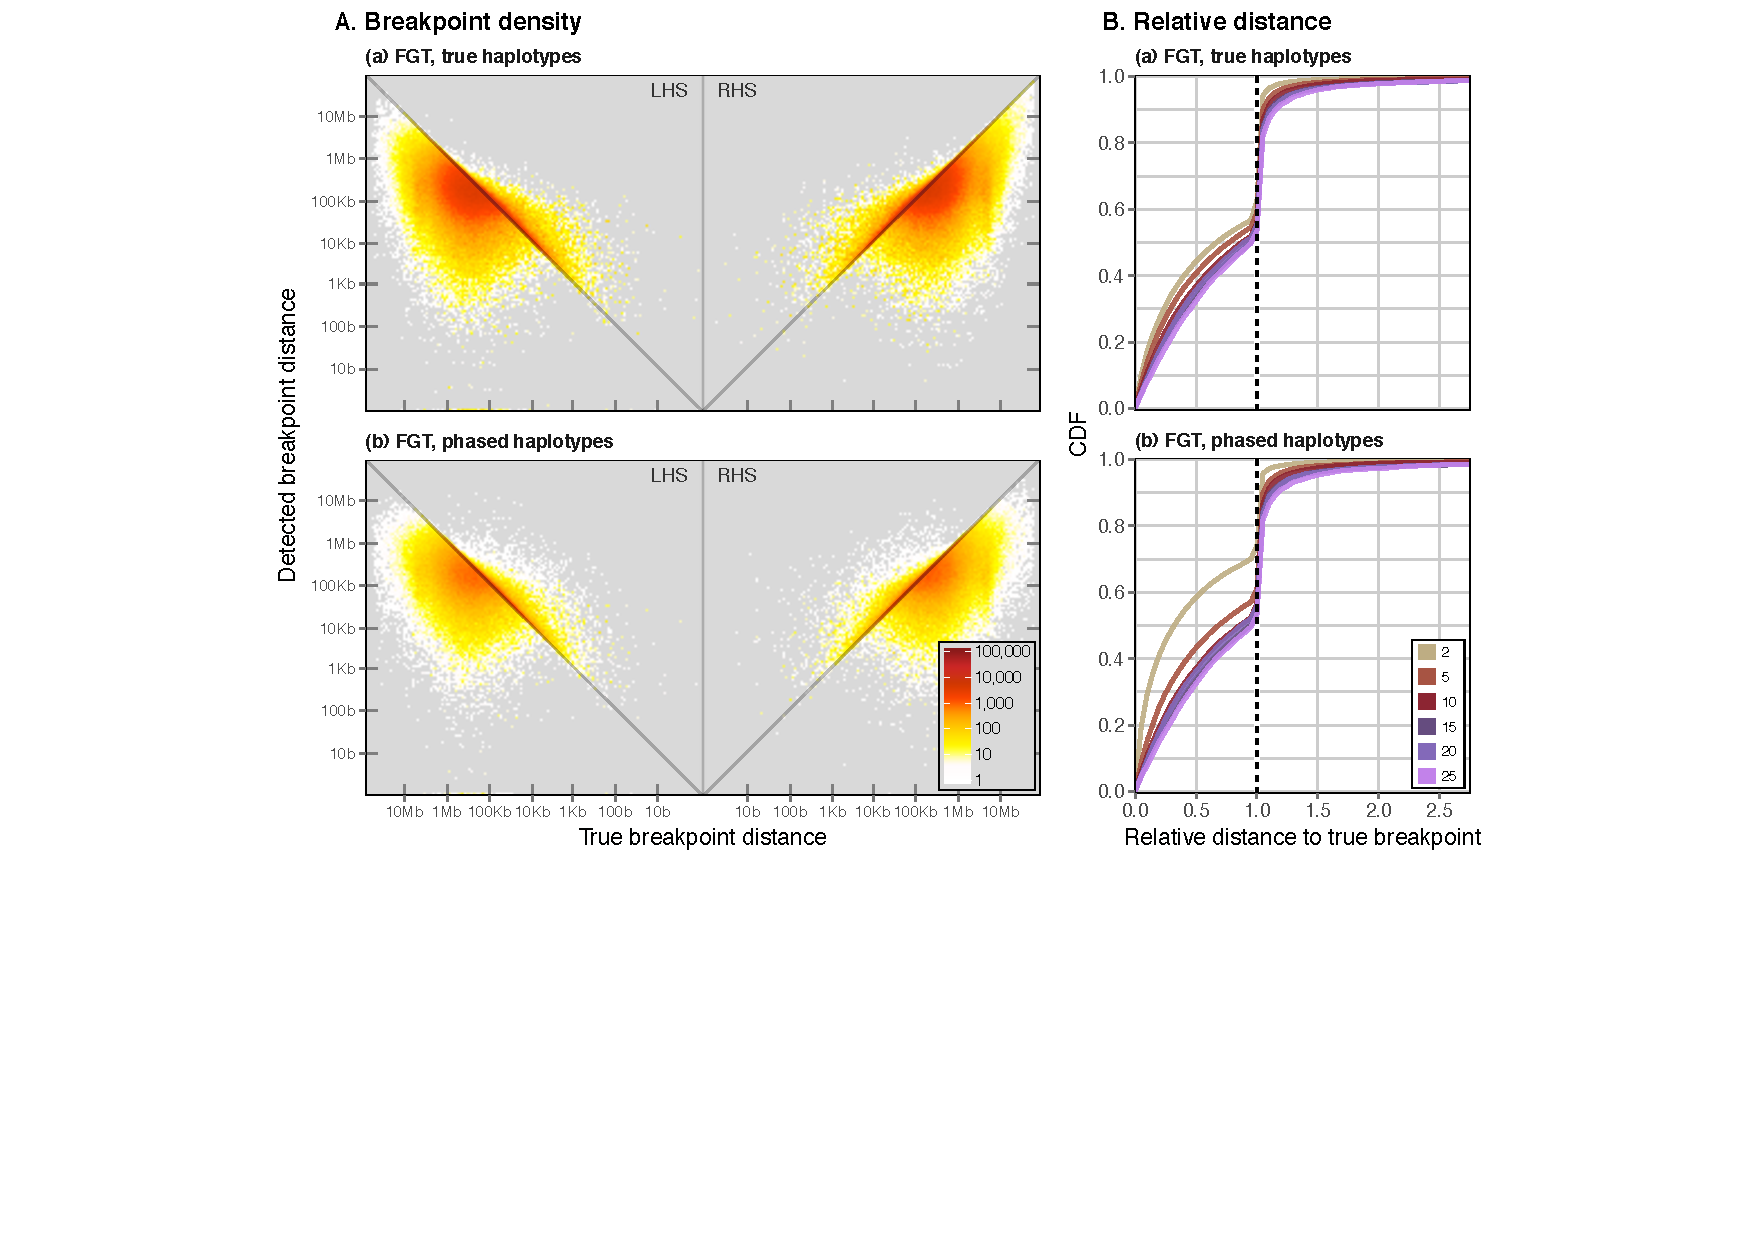
\includegraphics[width=\textwidth]{./img/ch3/beagle_break_tru}
\Caption{Accuracy of breakpoint detection in simulated data using Refined IBD in Beagle~4.1}
{Results are shown for uniquely detected shared haplotype segments inferred using the Refined IBD method; after removing boundary cases in either the detected or true segments, and after the detected segments were matched to the set of true segments.
Segments were inferred on true (simulated) haplotype data \textbf{(a)} and phased haplotypes \textbf{(b)}.
Panel~\textbf{(A)} provides a heatmap representation of a scatter plot, comparing physical distances between focal site and true breakpoint (x-axis) and detected breakpoint (y-axis).
Segment breakpoints to the left (\emph{LHS}) and right-and side (\emph{RHS}) of the focal position are shown separately.
Panel~\textbf{(B)} shows the \gls{cdf} of detected breakpoints in relative distance to the focal and true breakpoint sites.}
{fig:beagle_break_tru}
% \vspace{-5pt}
% \hrulefill%
\end{figure}
